\documentclass[12pt]{article}
\usepackage{amsmath} 
\usepackage{verbatim}
\usepackage{graphicx}    % For grafik (billederfiler)
\usepackage[T1]{fontenc} % For at blande \textsc{} med \textbf{}
\usepackage[dvipsnames,usenames]{color}
\usepackage{tabularx,colortbl,xcolor}
\definecolor{KU-red}{RGB}{144,26,30} 
\setlength{\parindent}{0mm}
\thispagestyle{empty}

\begin{document}

\begin{minipage}[b]{1.0\linewidth} 

\includegraphics[height=40mm]{KULogo}

\vspace*{-30ex}
\begin{center}
    {\Large \bf Project title} \vspace*{1ex} \\
    {\large ProjDat 2015} \vspace*{1ex} \\
    {\large Delrapport 1} \vspace*{1ex} \\
    {\large Emil Slot Arakelian Jensen - 170494} \vspace*{1ex}\\
    {\large Samuel Korn - 101186} \vspace*{1ex}\\
    {\large Mark Jay Nielsen - 250694} \vspace*{1ex}\\
    {\large Rune Bjerg Ono - 180187} \vspace*{1ex}\\
\end{center}

\vspace*{-3pt}
{\color{KU-red}\hrule}
\end{minipage}










\newpage

\tableofcontents










\newpage
\section{Problem definition}
\textbf{How many people are in the office?}\\
\textit{Use iBeacons to determine the amount of people currently in the office. Aggregate the data to apply machine learning and data visualizations.
Using iBeacons we would like to make an app that registers whenever the user enters or leaves our office. We would like to aggregate that data to use for cool data visualizations and applying machine learning to the data to obtain knowledge about the general usage patterns of the office. This could e.g. be used to adjust the heating, automatically lock the doors and turn off the lights when the last person leaves, predict when we need to order more or less lunch, or simply to check whether a certain person is currently at the office.} \cite{website}\\

The above text, is the original description of one of the many projects made available to us from the company Shape A/S.\\

On March the 12th, we had a meeting with S\o ren Ulrikkeholm, who is the developer responsible for student contact at Shape. We talked about the different projects and realistic acceptance criteria, taking into account our limited experience. We settled on the aforementioned project, because it was deemed the most appropriate for our level of skill, as well as being the one in which Shape had the most interest.\\

S\o ren explained that the company's biggest interest is learning how to use iBeacons with Android, with aggregation of the data and application of machine learning and data visualization are secondary objectives. We have decided to split the project into two development phases.\\

Our primary focus is on the first development phase, which consists of developing an app for Android that registers individual users entering and leaving the office space.\\

The second development phase consists of developing the backend for the system and integrating it with the app, in order to aggregate the data from users entering and leaving the office in a database.\\
A third phase, which we will not be working on, would be to apply machine learning and data visualizations to obtain knowledge about general usage patterns in the office.\\

In summation, our primary target is to deliver an Android app that is capable of registering data with the help of iBeacons. If there is enough time, our secondary target will be to develop the backend for this system. In both cases our deadline for delivery of the product has been set to June 8th 2015.\\










\section{Initial Software Project Management Plan}











\newpage
\section{Exercises}
\subsection*{1-8.}
\textbf{In the following description, explain when the term account is used as an application domain concept and when as a solution domain concept:}\\
"...managing bank accounts for mobile costumers." - It is used as an application domain concept, saying what it is supposed to do. 
"...provide access to the accounts when the..." - It is used the same way as before. 
"One proposal is that accounts are made available on the mobile computer..." - Here it is used as a solution domain concept, as it is a possible solution to be evaluated. 
"...the accounts show the amounts from the last connected session." - It is used in connection with the previous use.\\











\subsection*{2-6, 2-7, 2-9.}
\textbf{Draw a class diagram representing a book. Add multiplicity to the class diagram you produced in Exercise 2-6. Extend the class diagram to include attributes.}\\

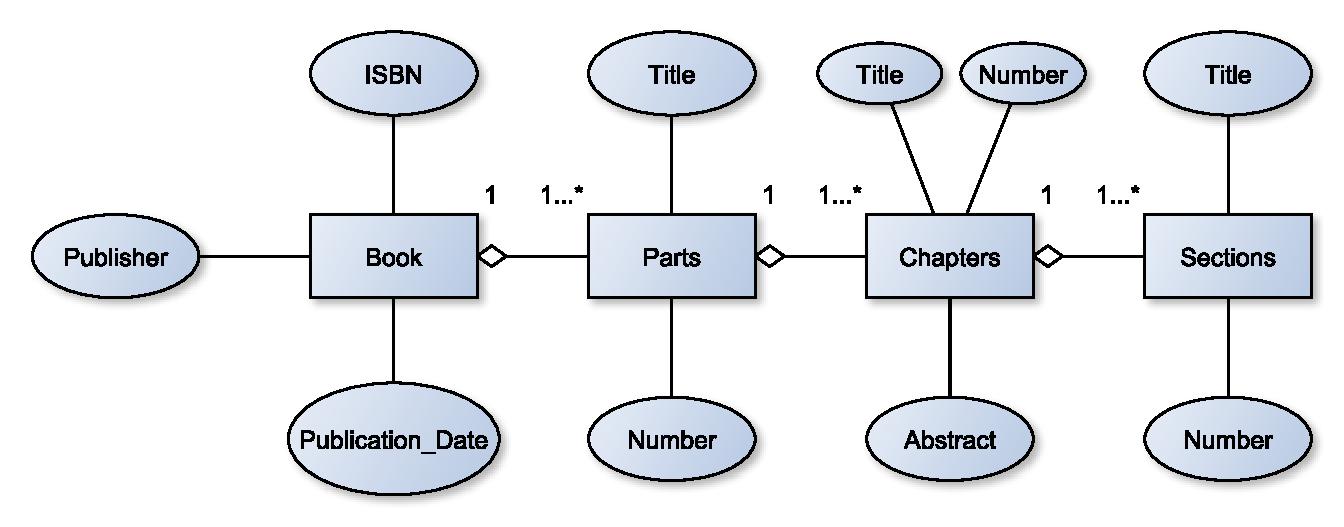
\includegraphics[height=50mm]{2-6}\\
\textbf{Fig 2:} Class diagram for exercise 2-6, 2-7 and 2-9








\newpage
\subsection*{2-10.}
\textbf{Add an abstract class and an inheritance relationship to factor out these two attributes into the abstract class}\\

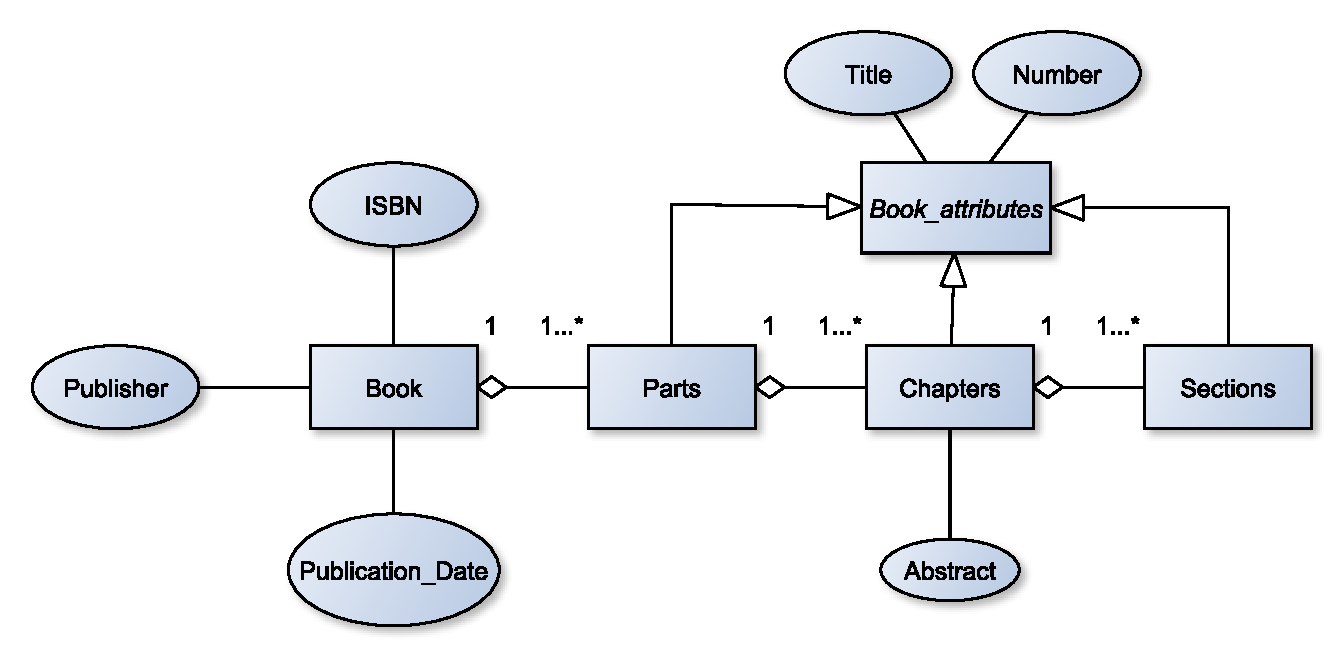
\includegraphics[height=70mm]{2-10}\\
\textbf{Fig 3:} Altered class diagram for exercise 2-10










\newpage
\subsection*{5-3.}
\textbf{Arrange the objects listed in Exercises 5-1 and 5-2 horizontally on a sequence diagram.}\\
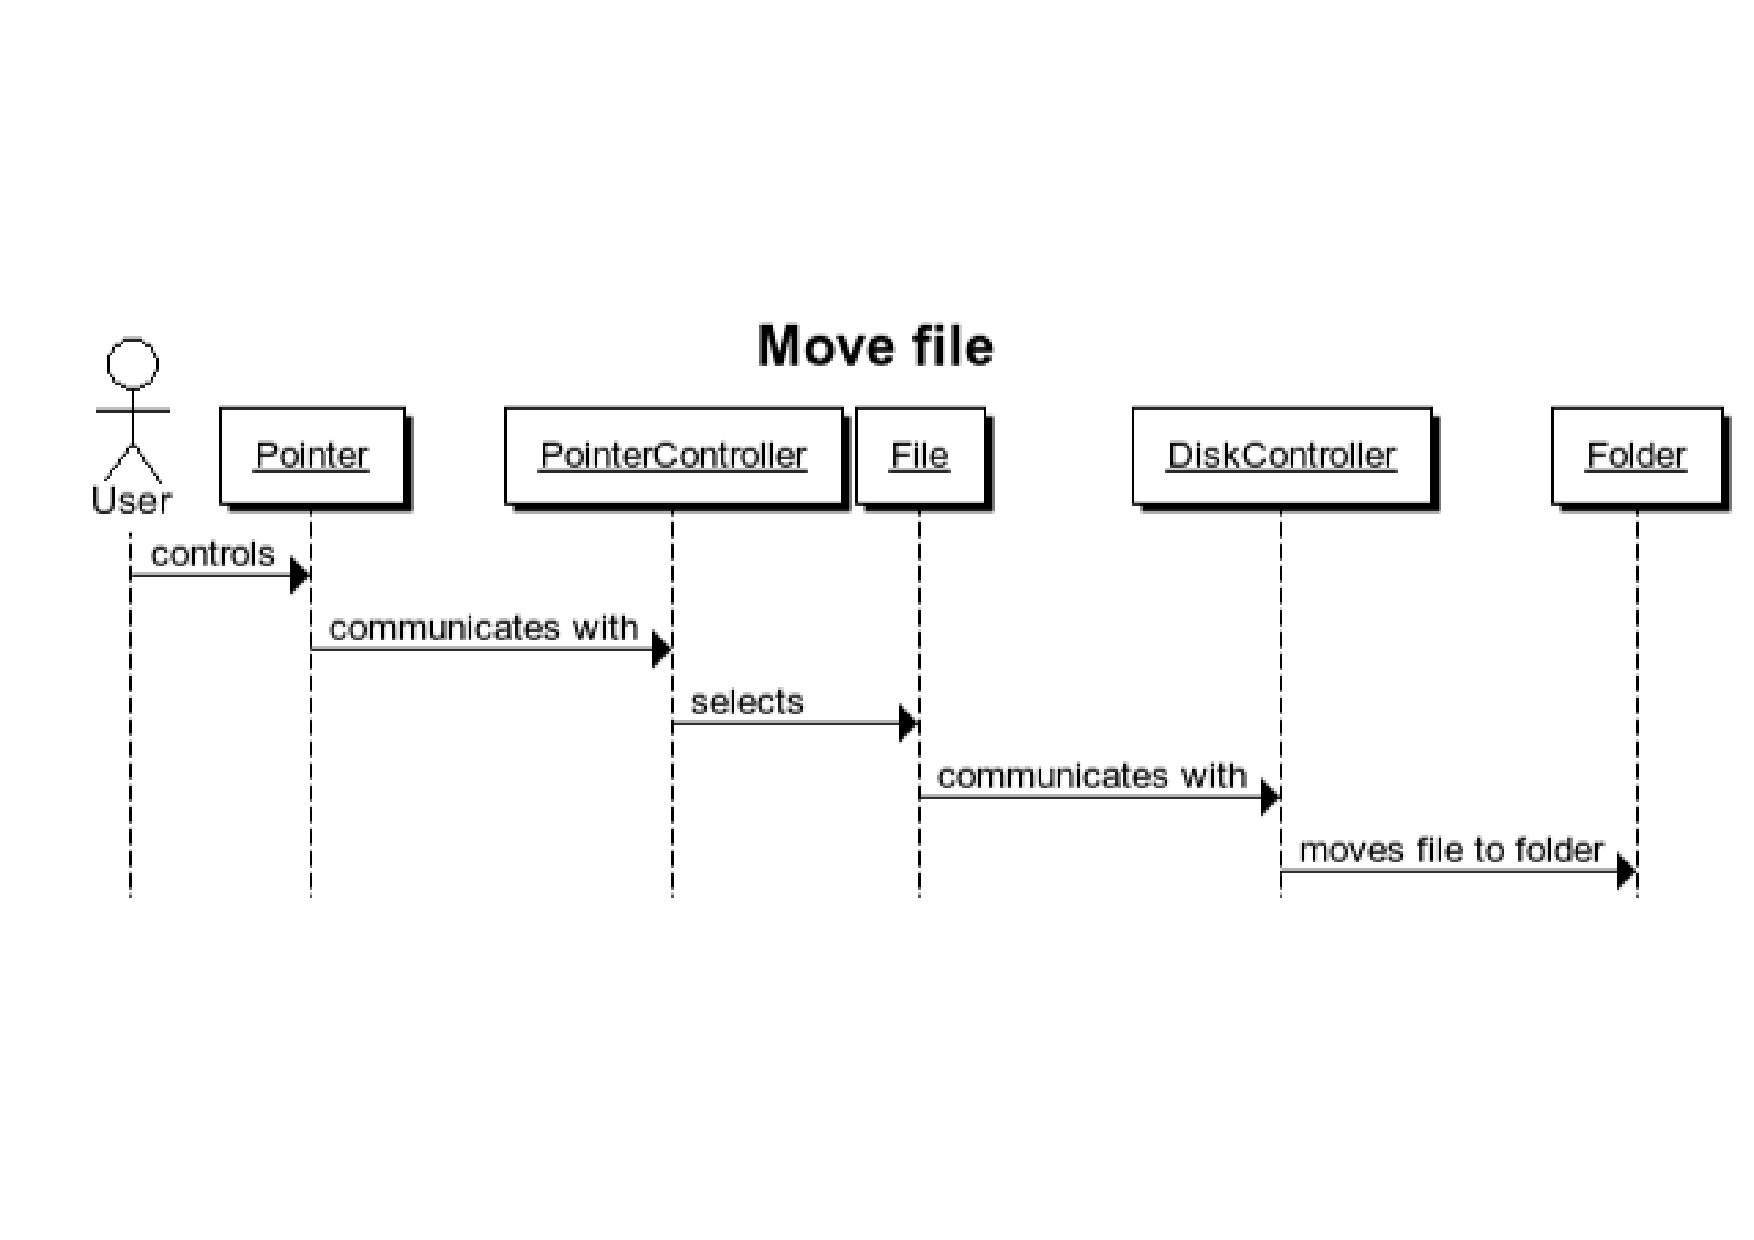
\includegraphics[scale=0.5]{5-3}\\
\textbf{Fig 4:} Sequence diagram for exercise 5-3


\newpage
\subsection*{7-1}
\textbf{Draw a UML deployment diagram representing the hardware/software mapping.}\\

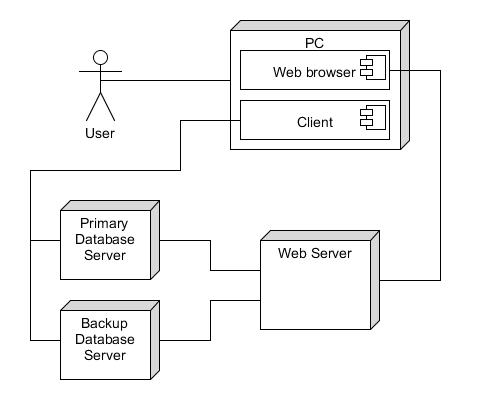
\includegraphics[scale=0.7]{7-1}\\
\textbf{Fig 5:} Deployment diagram for exercise 7-1







\newpage

\begin{thebibliography}{9}

\bibitem{website}
  www.shape.dk/projects

\end{thebibliography}

\end{document}
